% This file should contain text on the baseline design process and tools used by RVLT/Chris Silva for comparison to our new MDAO design process

% Add a description of the traditional process and tools used by Chris Silva and team for developing the 3 UAM vehicle designs.  Include an XDSM of the traditional process.  

% General outline for this section:
% \begin{itemize}
%     \item Traditional process used by RVLT for initial concept development applied different disciplinary tools in a linear/sequential fashion
%     \item NPSS used to create cycle model and engine surrogate model
%     \item CAMRAD used to model the rotors
%     \item ...tools for other disciplines...
%     \item NDARC used to determine mission performance
%     \item Optimization/iterations completed using this tool set to generate initial designs
%     \item Challenges:
%     \begin{itemize}
%         \item Process does not include detailed models for some disciplines (electrical?)
%         \item Existing tool set does not provide capabilities for completing large scale gradient-based optimization to further refine the designs
%     \end{itemize}
% \end{itemize}



The initial UAM concepts described in the Introduction were developed by the RVLT research team using a fairly traditional design process.
This process is generally described by the XDSM in Fig.~\ref{f:trad_XDSM} and can generally be described as a sequential execution of individual disciplinary design tools.
In the figure, three individual design disciplines are shown as an example, with the potential for adding additional disciplinary analyses as required

\begin{figure}[htb]
\begin{center}
 % \textbf{!!!!! Create XDSM of Traditional Process !!!!!}
 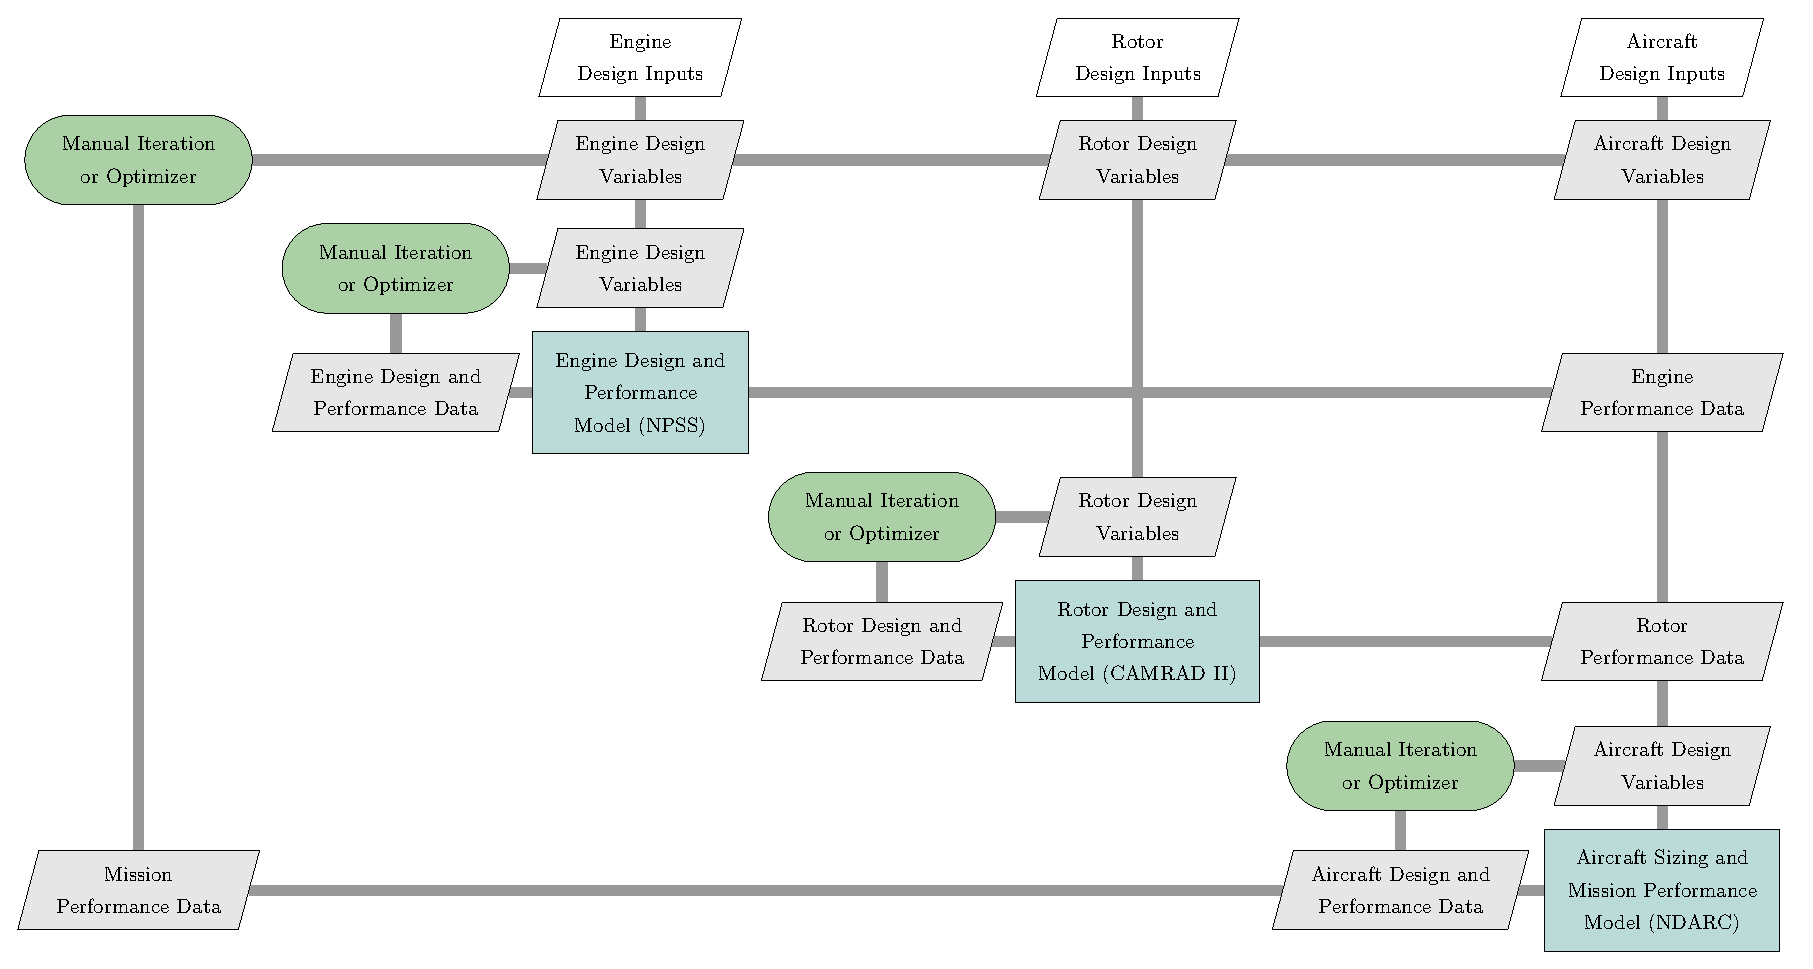
\includegraphics[width=1.0\textwidth]{../Images/Traditional_XDSM.pdf}
 \caption{Traditional Conceptual Design Process.}
 \label{f:trad_XDSM}
\end{center}
\end{figure}

The first discipline shown in this example process is for the turboshaft engine and commonly uses the Numerical Propulsion System Simulation (NPSS) code.\cite{claus1991numerical} 
This model both develops both the engine design and evaluates its performance over a wide range of operating conditions.
In the traditional process, a numerical optimizer or a series of manual iterations may be used to develop an engine suitable for the given aircraft and mission.
The result of this analysis is the generation of engine performance data with is required by later steps in the design process.
This data is often used to generate a data table or surrogate model that can be interpolated to determine performance characteristics for any feasible flight condition.

Next, a similar process is used to design the rotor(s) and determine the performance characteristics.
Within the RVLT project, this analysis is commonly completed using the Comprehensive Analytical Model of Rotorcraft Aerodynamics and Dynamics (CAMRAD II) code.\cite{johnson1994technology,johnson1998rotorcraft,johnson19981rotorcraft}
Like the engine analysis, design of the rotor(s) may include manual iterations or application of an optimizer to generate a desirable design
The resulting rotor performance data is also passed onto the last major disciplinary model.

The last disciplinary analysis model included in the generic process shown in Fig.~\ref{f:trad_XDSM} is for the overall aircraft design and mission performance evaluation.
This analysis develops and sizes the full vehicle then computes its performance over the mission(s) of interest and is commonly completed using the NASA Design and Analysis of Rotorcraft (NDARC) code.\cite{NDARC}
Like the previous disciplines, manual iterations or optimization can be used around the aircraft design and mission performance model to improve the design.
This vehicle design iteration/optimization typically occurs, however, without modification of the previously developed engine and rotor designs.
Therefore, if major limitations are the vehicle performance are uncovered an outer manual iteration or optimization loop might be required.  
This outer loop, represented by the green oval in the top left of the figure, would provided additional changes to the engine, rotor and aircraft design variables that would then need to be reevaluated through the entire process.

While this overall process and the constituent tools have historically worked well for developing conceptual rotorcraft designs, the traditional process has several weaknesses in regards to developing designs for emerging UAM vehicle concepts.
Primarily, the existing process centers around the sequential application of disciplinary tools to the design of the overall vehicle.
In this process, the individual disciplinary designs are developed in isolation with little understanding of how design changes will effect other disciplines or the overall system performance.
As a result, this sequential evaluation with loose coupling of the disciplines has been shown to produce suboptimal designs in other fields such as aerostructural analysis.\cite{Chittick:2007:B}
Furthermore, the sequential process becomes unwieldy as additional disciplinary analyses, such as electrical, thermal management, and acoustics which are vital for UAM concept development, must be include the design process.
The inclusion of several of these disciplines presents an additional challenge as the design requires a transient analysis of the disciplines and overall system.
This has been shown to be an issue for electrified propulsion systems where the heat generated by losses must be dissipated by a thermal management system with the performance depending on the operating time history.\cite{falck_electric_thermal_2017}






-Moving to unconventional systems/configurations which aim to apply emerging technologies and take advantage of disciplinary interactions to improve the performance\\
-This includes the use of electrified propulsion systems\\

Also makes assumptions about the operating characteristics (flight path) that could be non-ideal for new technologies

Process does not include detailed models for some disciplines (electrical, TMS, acoustics?)
Existing tool set does not provide capabilities (specifically accurate analytic or semi-analytic derivatives) for completing large scale gradient-based optimization to further refine the designs

Economics of UAM vehicles will be important for long term viability






Sequential process with weak coupling between disciplines that were designed/optimized in isolation
Subsystem design/optimization becomes more unwieldy as more disciplines are added and does not generally lead to overall optimal design (cite Martins)


Sequential process (cite martins)
-no passing of impact of changes on constraints

Transient analysis (cite X57)


Challenge of tightly integrating existing tools
-Computational cost goes up
-Complexity of model goes up
-Numerical stability of analysis drops
    -computation of derivatives
    -likelihood of code failing

mission/transient analysis is challenging




